\documentclass[11pt,oneside,brudnopis]{xelatex-mgr/xmgr}

\usepackage{amsmath}
\usepackage{blindtext}

%\defaultfontfeatures{Scale=MatchLowercase}
%\setmainfont[Numbers=OldStyle,Ligatures=TeX]{Minion Pro}
%\setsansfont[Numbers=OldStyle,Ligatures=TeX]{Myriad Pro}
% for fontspec version < 2.0
% \setmainfont[Numbers=OldStyle,Mapping=tex-text]{Minion Pro}
% \setsansfont[Numbers=OldStyle,Mapping=tex-text]{Myriad Pro}
\setmonofont[Scale=0.75]{Monaco}

\wersja   {wersja wstępna [\ymdtoday]}

\author   {Bartłomiej Kruczyk}
\nralbumu {213603}
\email    {bartlomiej.kruczyk@gmail.com}

\title    {Efektywne algorytmy dla wielokątów wypukłych}
\date     {2014}
\miejsce  {Gdańsk}

\opiekun  {dr Paweł Żyliński}

\begin{document}

\begin{abstract}
\blindtext[1]
\end{abstract}

\keywords{}

\maketitle

% \introduction

\chapter{Podstawowe pojęcia}
W tym miejscu zostaną przybliżone podstawowe pojęcia związane z
geometrią obliczeniową i problemami dotyczącymi wielokątów wypukłych.

\begin{itemize}
\item{\emph{wielokąt wypukły}} --- wielokąt prosty którego wnętrze
  jest zbiorem wypukłym: wszystkie punkty należące do odcinka
  łączącego dwa dowolne punkty ze zbioru wypukłego należą do tego
  zbioru

  \begin{figure}[htp]
    \centering
    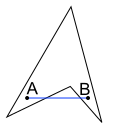
\includegraphics{img/nonconvex}
    \caption{Figura niebędąca wielokątem wypukłym.}
  \end{figure}

\item{\emph{średnica zbioru punktów}} --- średnicą zbioru punktów
  nazywamy największą odległość pomiędzy dwoma punktami należącymi do
  zbioru

\item{\emph{lewoskrętność, prawoskrętność}} --- o kącie mówimy, że
  jest lewoskrętny jeżeli wyznacznik $3 \times 3$ współrzędnych punktów
  $p_1$, $p_2$, $p_3$ kąta jest dodatni, w przeciwnym przypadku
  mówimy, że kąt jest prawoskrętny. Jeżeli $p_i = (x_i, y_i)$ to
  wyznacznik:

  \begin{center}
    \begin{math}
      \begin{vmatrix}
        x_1 & y_1 & 1 \\
        x_2 & y_2 & 1 \\
        x_3 & y_3 & 1
      \end{vmatrix}
    \end{math}
  \end{center}

\item{\emph{proste wspierające}} --- prostymi wspierającymi dla wielokąta
  nazywamy takie proste, które przechodząc przez wierzchołek wielkąta
  nie przecinają jego wnętrza

\item{\emph{punkty antypodyczne}} --- taka para wierzchołków wielokąta przez
  które można poprowandzić równoległe proste wspierające

\item{\emph{notacja wielkiego O}} --- notacja asymptotycznego tempa
  wzrostu wartości funkcji względem jej argumentów, w algorytmice
  stosowana do charakterystyki złożoności obliczeniowej algorytmów
  opisując ilość potrzebnych zasobów (czasu lub pamięci) w stosunku do
  rozmiaru danych wejściowych. Mówimy, że funkcja $f$ jest co najwyżej
  rzędu $g$ (jest ograniczona przez funkcję $g$), gdy istnieją takie
  stałe $n_0 > 0$ oraz $c > 0$, takie że:

  \begin{center}
    $\forall n \geq n_0 : f(n) \leq c \cdot g(n)$
  \end{center}

  \begin{table}[htp]
    \centering
    \caption{Najczęściej wyróżniane rzędy żłożoności obliczeniowej,
      podane według rosnącej złożoności.}
    \begin{tabular}{c c}
      $O(1)$ & stała \\
      \hline
      $O(\log n)$ & logarytmiczna \\
      \hline
      $O(n)$ & liniowa \\
      \hline
      $O(n \log n)$ & liniowo-logarytmiczna \\
      \hline
      $O(n^2)$ & kwadratowa \\
      \hline
      $O(n^c)$ & wielomianowa \\
      \hline
      $O(c^n)$ & wykładnicza \\
      \hline
      $O(n!)$ & ograniczona przez silnię \\
    \end{tabular}
  \end{table}

  W tej pracy efektywnym algorytmem będziemy nazywać algorytm o
  złożoności nie większej niż liniowo-logartymiczna.
\end{itemize}

\chapter{Przegląd problemów}
Przedstawione w niniejszym rozdziale problemy są wspólne dla
wszystkich wielokątów, co pozwala na porównanie rozwiązań i ich
efektywności dla wielokątów prostych i wypukłych. Przy każdym
problemie zostanie przedstawione rozwiązanie naiwne, następnie
rozwiązanie dla wielokąta wypukłego wraz z analizą złożoności oraz
w miare możliwości dowodem poprawności algorytmu.

\section{Lokalizacja punktu}

% \section{Średnica wielokąta}
% \section{Przecięcie wielokątów}
% \subsection{Shamos --- Hoey}
% \subsection{O'Rourke --- Nador}
% \subsection{Separating Axes}
% \section{Zawieranie wielokątów}
% \section{Wyznaczanie prostokąta zawierającego wielokąt}
% \section{Wyznaczanie największej odległości między wielokątami}
% \section{Złączanie wielokątów wypukłych}
% \section{Znajdowanie krytycznych linii wsparcia}

% \summary

% \appendix
% \chapter{Generowanie wielokątów wypukłych o zadanej liczbie
%   wierzchołków}

% \bibliographystyle{unsrt}
% \bibliography{xml}

% \listoftables

% \listoffigures

% \oswiadczenie

\end{document}

%%% Local Variables:
%%% coding: utf-8
%%% mode: latex
%%% TeX-master: t
%%% TeX-engine: xetex
%%% End:
